\chapter{Introduction}

This chapter frames the problem of secure and anonymous electronic voting and explains why a blockchain-backed approach is explored. It situates the project within the context of privacy risks, auditability requirements, and accessibility needs. It also introduces the local-chain approach as a practical implementation path for edge environments. The chapter concludes by defining the scope of the work and how the proposed flow addresses key limitations.

\section[Introduction]{\textbf{Introduction}}
Electronic voting systems have evolved significantly over recent decades, yet the twin challenges of preserving voter privacy and ensuring result integrity remain largely unsolved. Many deployed systems continue to rely on centralized databases or direct vote logging, which exposes voters to identity-to-choice linkage and creates single points of failure for tampering. Blockchain technology offers immutability and public auditability as potential remedies, but a naive on-chain design introduces timing correlations and direct vote mapping that undermine anonymity. This project investigates a hybrid architecture that combines identity hashing, batched and shuffled submission, and local-chain deployment to address these gaps while remaining practically deployable.

\section[Literature Review]{\textbf{Literature Review}}
A literature review surveys the current body of knowledge relevant to a topic, synthesizing substantive findings and theoretical or methodological contributions from prior work. The following reviews examine research in blockchain standardization, authentication protocols, verifiable online voting, and privacy-preserving data collection — areas that collectively inform the design of the proposed system. Each paper is reviewed for its core findings and their relevance to the present project.

\subsection{Review of Related Works}

\subsubsection{\textbf{Blockchain Standardization and Regulation}}
Fardad and Mohammadzadeh Mianji \cite{Fardad2025} examine the landscape of blockchain and distributed ledger technology standardization...

\subsubsection{\textbf{Authentication in Constrained Systems}}
Hosseinzadeh and Servati \cite{Hosseinzadeh2024} evaluate two proposed ultra-lightweight RFID authentication protocols...

\subsubsection{\textbf{End-to-End Verifiable Online Voting}}
Alsadi and Casey \cite{Alsadi2024} address the lack of transparency and verifiability...

\subsubsection{\textbf{Differential Privacy on Blockchain}}
Wang and Zhu \cite{Wang2023} contrast private and public blockchain architectures...

\section[Motivation]{\textbf{Motivation}}
Privacy-preserving voting is essential for democratic integrity and public trust...

\section[Problem Statement]{\textbf{Problem Statement}}
The core problem is to prevent linkage between voter identity and candidate choice...

\section[Objectives]{\textbf{Objectives}}
The objective of this project is to design and implement a privacy-preserving electronic voting system...

\section[Brief Methodology of the project]{\textbf{Brief Methodology of the project}}
\begin{enumerate}
    \item Voter identity is hashed at registration to decouple identity from the voting record.
    \item Cast votes are stored in a local buffer before submission.
    \item Votes are shuffled and submitted as a batch to reduce timing correlation.
    \item The batch is written to the local blockchain to ensure immutability and auditability.
    \item Aggregated results are displayed without exposing individual vote mappings.
\end{enumerate}

\begin{figure}[htbp]
    \centering
    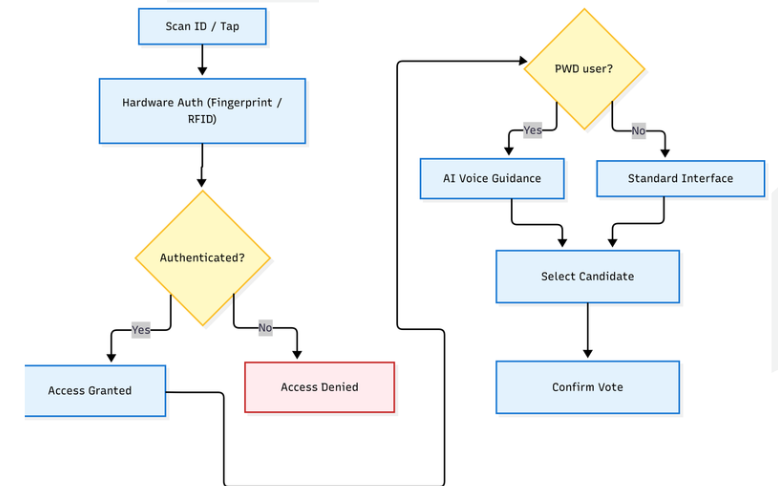
\includegraphics[width=0.8\linewidth]{Chapter1/1.png}
    \caption{Methodology Flow}
    \label{fig:methodology}
\end{figure}
\newpage
\section[Assumptions made / Constraints of the project]{\textbf{Assumptions made / Constraints of the project}}
The following assumptions and constraints apply to the current phase of the project:
\begin{itemize}
    \item The system operates on a local (private) blockchain; public chain deployment is outside the current scope.
    \item Hardware-backed identity verification (e.g., biometrics, smart cards) is not included in this phase.
    \item The voter device is assumed to be trusted; client-side malware is outside the threat model.
    \item Network connectivity is assumed only within the local deployment environment.
    \item The prototype is evaluated for functional correctness and anonymity properties; formal cryptographic proofs are deferred to future work.
\end{itemize}

\section[Organization of the Report]{\textbf{Organization of the Report}}
This report is organized as follows.
\begin{itemize}
    \item Chapter 1 introduces the project, reviews relevant literature, states the problem, and defines the scope and objectives.
    \item Chapter 2 discusses the fundamentals of blockchain technology and the privacy properties relevant to electronic voting.
    \item Chapter 3 discusses the system architecture, including identity hashing, batch shuffling, and local-chain design.
    \item Chapter 4 discusses the implementation of the voting flow and the dual-interface client.
    \item Chapter 5 discusses future work and scope of the project.
\end{itemize}